% Appendix A: AHSD backbone (reviewer request). Values from src/nids/models/ahsd.py (variant "fixed"),
% src/nids/train.py and configs/data.yaml.
\appendices
\section{AHSD backbone}
\label{app:ahsd}

AHSD (adaptive homeostatic sequence detector) is the recurrent backbone that produces the confidence and representation scores. It was designed for this study and is used only in its \emph{fixed} variant, in which the benign reference $E$ does not change within a window (Fig.~\ref{fig:ahsd}). Its core idea is homeostasis: the state $h_t$ starts at the benign reference, is pulled toward each new embedding by the gate $\alpha_t$ and relaxed back toward the reference by $\beta_t$, so traffic that keeps the state away from $E$ produces a large \emph{stress}.

\begin{figure*}[!t]
\centering
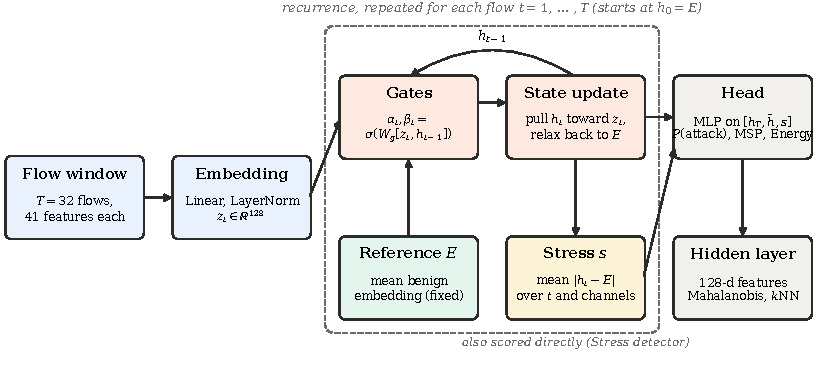
\includegraphics[width=\textwidth]{fig_ahsd_arch.pdf}
\caption{AHSD architecture (fixed variant). The recurrence inside the dashed frame runs once per flow of a 32-flow window, starting from $h_0=E$. The head reads the last state, the mean state and the stress $s$; its output gives $P(\text{attack})$, MSP and energy, and its 128-d hidden layer feeds Mahalanobis and $k$NN.}
\label{fig:ahsd}
\end{figure*}

\noindent\fbox{\begin{minipage}{\dimexpr\columnwidth-2\fboxsep-2\fboxrule\relax}
\small
\textbf{Algorithm 1:} AHSD forward pass (fixed variant)\\[2pt]
\textbf{Input:} window $x_1,\dots,x_T$ ($T=32$ flows, $F$ features); reference $E\in\mathbb{R}^{D}$, $D=128$\\
\textbf{Output:} $P(\text{attack})$, stress $s$, hidden vector $u$\\[-6pt]
\begin{enumerate}\setlength{\itemsep}{0pt}\setlength{\leftmargini}{14pt}
\item $h_0 \leftarrow E$
\item \textbf{for} $t=1,\dots,T$ \textbf{do}
\item \quad $z_t \leftarrow \mathrm{LayerNorm}(W x_t + b)$
\item \quad $[\alpha_t,\beta_t] \leftarrow \sigma\big(W_g[z_t,h_{t-1}] + b_g\big)$
\item \quad $h_t \leftarrow h_{t-1} + \alpha_t\odot(z_t-E) - \beta_t\odot(h_{t-1}-E)$
\item $s \leftarrow \frac{1}{TD}\sum_{t,d}|h_{t,d}-E_d|$
\item $u \leftarrow \mathrm{GELU}\big(W_1[h_T,\ \tfrac{1}{T}\textstyle\sum_t h_t,\ s] + b_1\big)$
\item $P(\text{attack}) \leftarrow \mathrm{softmax}(W_2 u + b_2)_{\text{attack}}$
\end{enumerate}
\end{minipage}}
\medskip

\textbf{Reference $E$.} During training, $E$ is an exponential moving average (momentum 0.01) of the embeddings $z_t$ of benign windows in each batch. After training it is set exactly to the mean embedding of the benign training windows and then kept fixed. It is not a learned parameter.

\textbf{Training.} Windows of $T=32$ consecutive flows (stride 16) are labelled attack if any flow is an attack. Training sets are balanced 1:1, and the loss is cross-entropy on the two classes. We use AdamW (learning rate $10^{-3}$, weight decay $10^{-4}$) with a cosine schedule, gradient clipping at 1.0, batch size 256 and 15 epochs, and keep the checkpoint with the best validation macro-F1. No hyperparameter is tuned per dataset or detector.

\textbf{Size.} With the $F=41$ features of D1--D3, AHSD has 104,706 parameters: 5,632 in the embedding (linear and LayerNorm), 65,792 in the gates ($2D\!\to\!2D$) and 33,282 in the head ($2D{+}1\!\to\!D\!\to\!2$). The GRU control (Sec.~\ref{sec:s3}) replaces the gated recurrence with a one-layer GRU of hidden size 128, keeps the same embedding and head without stress, and is trained identically.

\textbf{Scores.} $P(\text{attack})$, MSP and energy are computed from the head output; stress is the value $s$; Mahalanobis and $k$NN distances are computed on the hidden vector $u$, with benign training windows as the reference set.
